\newpage
\section{Introducción}
\vspace{0.3cm}

En la actualidad, el concepto de red convencional energética está siendo transformado como resultado del creciente auge de las redes inteligentes de energía (del inglés Smart Grids, \textbf{SG}). La posibilidad de monitorizar a tiempo real el proceso de distribución eléctrica de una forma eficiente y de integrar a la vez una participación activa del consumidor, convierte a estas redes en uno de los pilares fundamentales de la transición hacia la descarbonización. Es por ello que, en este contexto, la búsqueda de nuevos protocolos de encaminamiento y distribución energética se ha vuelto primordial. 

\vspace{0.3cm}

Desde el equipo de investigación NetIS de la Universidad de Alcalá (\textbf{UAH}) se ha diseñado \textbf{DEN2NE} (Distributed ENergy ENvironments and Networks), un nuevo algoritmo para automatizar la gestión de los recursos en entornos de El Internet de las Cosas (del inglés Internet of Things, \textbf{IoT}) y, en particular, en Smart Grids. En este último caso, el objetivo principal del algoritmo se basa en conseguir un balance energético global de la red. Se encarga de realizar una distribución óptima de los recursos entre los diferentes nodos, que toman el papel de prosumidores, siendo capaces tanto de consumir como de producir energía a partir de fuentes renovables.

\vspace{0.3cm}

No obstante, actualmente \textbf{DEN2NE} aún presenta como desafío a afrontar la necesidad de detectar y predecir de una forma precisa los posibles fallos que se pueden producir en el proceso de intercambio energético. Adicionalmente, en caso de error, el algoritmo debería ser capaz de definir una respuesta rápida para tomar acciones a nivel de distribución y evitar que el problema escale al resto de la red.

\vspace{0.3cm}

\section{Objetivos y campos de aplicación}
\vspace{0.3cm}

El objetivo principal de este proyecto consiste en desarrollar diferentes técnicas de aprendizaje automático (del inglés machine learning, \textbf{ML}) para identificar las circunstancias o motivos por las que se pueden producir fallos en una Smart Grid durante el proceso de distribución energética que lleva a cabo el algoritmo \textbf{DEN2NE}. La identificación de patrones se basará en el análisis de grandes volúmenes de datos provenientes de medidores (smart meters) y sensores implementados en Smart Grids reales. Finalmente, la aplicación de diferentes métodos basados en inteligencia artificial (IA) permitirá determinar un modelo preciso de predicción de fallos. Se pueden sintentizar los diferentes objetivos del proyecto en los siguientes puntos:

\begin{itemize}
    \item Estudio del estado del arte y análisis de las diferentes fuentes de datos reales disponibles.
    \item Definición y procesado del volumen de datos para el posterior desarrollo. 
    \item Planteamiento de diferentes escenarios.
    \item Generación y simulación de topologías.
    \item Desarrollo y entrenamiento de diferentes modelos de machine learning (ML).
    \item Análisis de los resultados obtenidos.
\end{itemize}

\vspace{0.3cm}

\section{Descripción del trabajo}
\vspace{0.3cm}

El desarrollo del trabajo fin de máster (TFM) se ha dividido en distintas etapas. La primera se basará en estudiar en profundidad el contexto en el que se engloban las redes inteligentes de energía y el funcionamiento de los protocolos de distribución de recursos, enfocando el análisis en \textbf{DEN2NE} como se ha mencionado anteriormente. Además, será preciso investigar sobre las diferentes fuentes de datos disponibles provenientes de implementaciones reales y valorar su viabilidad para este proyecto. 

\vspace{0.3cm}

Por consiguiente, cuando se hayan adquirido los suficientes conocimientos sobre el estado del arte, será necesario analizar y evaluar el volumen de datos que será necesario para llevar a cabo el desarrollo de los patrones de error. En esta etapa será necesario un procesado exhaustivo de los datos con el fin de simplificar su comprensión.

\vspace{0.3cm}

Una vez realizado este proceso, se habrá definido un número determinado de parámetros iniciales que se podrán asignar a los diferentes nodos de una red. A partir del volumen de datos elaborado, se plantearán una serie de escenarios y se generarán diversas topologías aleatorias mediante la herramienta BRITE. Estas serán posteriormente importadas a un simulador propietario realizado en Python. Los resultados de las diferentes pruebas realizadas proporcionarán finalmente el conjunto de datos necesario para el entrenamiento de los modelos a desarrollar.

\vspace{0.5cm}

\begin{figure}[!htb]
  \centering
  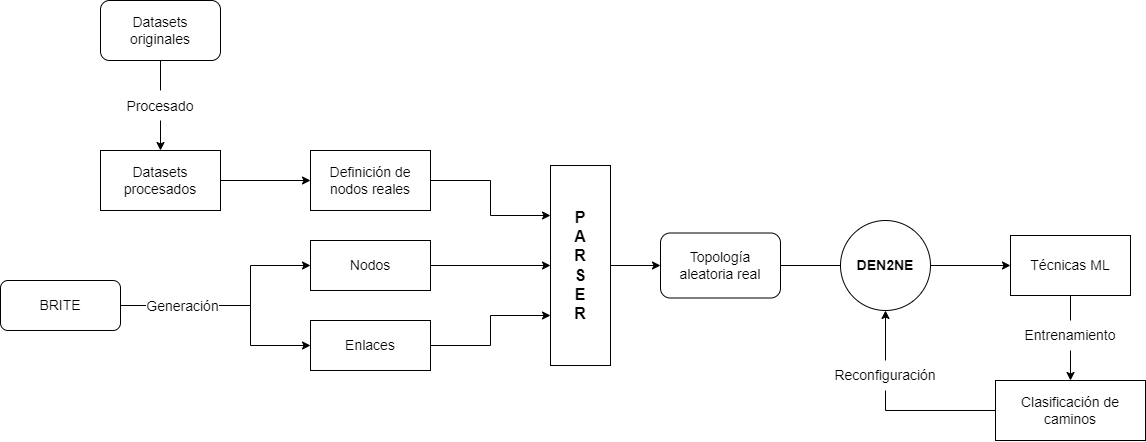
\includegraphics[width=1\textwidth]{img/imagen.drawio.png}
  \caption{Proceso de detección y predicción de errores}
  \label{fig:1}
\end{figure}

\vspace{0.3cm}

Como se viene introduciendo, la siguiente etapa consistirá en el desarrollo de varias técnicas de machine learning para la búsqueda de patrones de error a partir de los datos procesados. En primera instancia, será necesaria una valoración de los modelos más apropiados a emplear, teniendo en cuenta el contexto en el que se encuentra el proyecto. El desarrollo y entrenamiento progresivo de cada uno de ellos dará lugar a unos resultados de predicción determinados que serán probados y analizados. En base a la precisión obtenida de este proceso, se podrá determinar de forma concluyente el modelo de machine learning con mayor efectividad para poder diagnosticar errores en una Smart Grid. 

\vspace{0.3cm}

\section{Metodología y plan de trabajo}
\vspace{0.3cm}
\begin{itemize}

\item \textbf{Documentación y estudio:} Establecimiento de los conocimientos necesarios y definición del estado del arte a través de la búsqueda y recolección de información, artículos y papers científicos.  

\item \textbf{Planificación:} Elaboración de los hitos que se pretenden conseguir con este proyecto. Planteamiento del organigrama del workflow a seguir y definición de las diferentes fases del desarrollo software.

\item \textbf{Análisis y tratamiento de datos:} Investigación sobre diferentes implementaciones de redes inteligentes reales, evaluación de su viabilidad para este proyecto y procesado exhaustivo del conjunto de datos disponible.

\item \textbf{Elaboración de escenarios:} Establecimiento de diferentes escenarios y generación de las topologías a simular mediante la herramienta BRITE.  

\newpage

\item \textbf{Simulación:} Simulación de las topologías generadas para la obtención del volumen de datos definitivo que se pretende entrenar.

\item \textbf{Desarrollo y entrenamiento de modelos:} Selección de varias técnicas de ML acorde a las necesidades del proyecto y, por consiguiente, desarrollo software y entrenamiento progresivo de los modelos.

\item \textbf{Análisis de efectividad:} Validación de las técnicas desarrolladas y elaboración de un análisis concluyente en base a los resultados obtenidos y a su precisión. 

\item \textbf{Informe final:} Redacción de un informe que recoja toda la documentación necesaria respectiva al estudio, desarrollo y análisis de este proyecto.

\end{itemize}

\vspace{0.3cm}

La metodología que se propone para la realización del proyecto es la de Proceso Unificado enfocado al desarrollo de software, la cual se caracteriza por estar dirigido por casos de uso o emulaciones, centrado en la arquitectura del sistema y por ser iterativo e incremental. En este proyecto, según se podrá apreciar en la Planificación del TFM (Sección \ref{sec:planificacion}), se plantean múltiples iteraciones, en las cuales se pasará de forma secuencial por las siguientes etapas:

\begin{itemize}
    \item \textbf{Diseño del entorno} 
    \item \textbf{Desarrollo de modelos ML}
    \item \textbf{Validación del desarrollo}
\end{itemize}

\vspace{0.3cm}

\section{Planificación del TFM}
\label{sec:planificacion}
\begin{figure}[htb]
\begin{center}

\begin{ganttchart}[
	hgrid,
	vgrid,
	y unit chart=.8cm,
	bar/.append style={fill=cyan!50},
	expand chart=\textwidth
	]{1}{15}
\gantttitle{Semanas}{15} \\
\gantttitlelist{1,...,15}{1} \\
\ganttbar{Documentación y estudio}{1}{3} \\
\ganttbar{Planificación}{1}{3} \ganttnewline
\ganttbar{Análisis y tratamiento de datos}{3}{5} \ganttnewline
\ganttbar{Elaboración de escenarios}{4}{5} \ganttnewline
\ganttbar{Simulación}{5}{6} \ganttnewline
\ganttbar{Desarrollo y entrenamiento de modelos}{5}{12} \ganttnewline
\ganttbar{Análisis de efectividad}{11}{12} \ganttnewline
\ganttbar{Informe final}{13}{15}
\end{ganttchart}

\end{center}
\caption{Diagrama de Gantt del proyecto}
\end{figure}



\section{Medios}

\vspace{0.3cm}
En cuanto a los medios hardware, para el desarrollo de este proyecto se estima principalmente el empleo de un ordenador portátil. Es importante que este cuente con la suficiente capacidad de memoria RAM y de procesador para poder llevar a cabo el desarrollo software del proyecto de una manera fluida.

\vspace{0.3cm}
Por otro lado, en cuanto a las herramientas software, se empleará \textit{GIT} para llevar a cabo el control de versiones del proyecto y Visual Studio Code como editor de código fuente. Adicionalmente, se utilizará BRITE como herramienta de generación de topologías aleatorias.

\newpage
